\documentclass[UTF8]{ctexart}
\usepackage{lmodern}
\usepackage{amsmath}
\usepackage{amssymb}
\usepackage{graphicx}
\usepackage{geometry}
\usepackage{float}
\usepackage{color}
\geometry{left=2.18cm,right=2.18cm,top=1.54cm,bottom=2.0cm}
\pagestyle{empty}
\title{\textbf {2025秋计算方法--实验报告 \#4---16分(小结占2分)}}
\author{\textbf{姓名：金天昊 \quad 学号：PB24000144}}
\date{\today}

\begin{document}

\maketitle

运行环境：Windows 11, VSCode, CPython 3.13.6
%win11，vscode，py3

\section*{实验内容与要求}

    对函数\textcolor{blue}{~$f(x)=\dfrac{7x+3}{x^2-2x+7},x\in[-5,5]$},
    构造其$N$次\textcolor{blue}{Lagrange插值函数} $p(x)$, \\
    取~$\color{blue}\max\limits_{x\in[-5,5]}|f(x)-p(x)|\approx\max\limits_{0\leq i\leq 500}|f(y_i)-p(y_i)|,y_i=\dfrac{i}{50}-5$~为\textcolor{blue}{近似插值误差},\\
    分别取如下两种\textcolor{blue}{插值节点}~(\textcolor{red}{均为~$N+1$个})：

    \begin{enumerate}
        \item $\color{blue}x_i=-5+\dfrac{10}{N}i,~~i=0,1,\cdots,N$~~(均匀节点)
        \item $\color{blue}x_i=-5\cos\left(\dfrac{2i+1}{2N+2}\pi\right),~~i=0,1,\cdots,N$~~(Chebyshev点).
    \end{enumerate}

    分别取~\textcolor{blue}{$N=4,8,16,32$}, 画出两种插值效果的对比函数图像(包括~$f(x)$的图像),
    列表给出以上两组节点的插值误差结果（保留到小数点后12位）;
    针对插值结果, 作出适当的分析与小结.



\section{数值结果(须包含插值效果对比图)}
两种节点的插值效果图分别如图1--图4所示。

\begin{figure}[H]
	\centering
	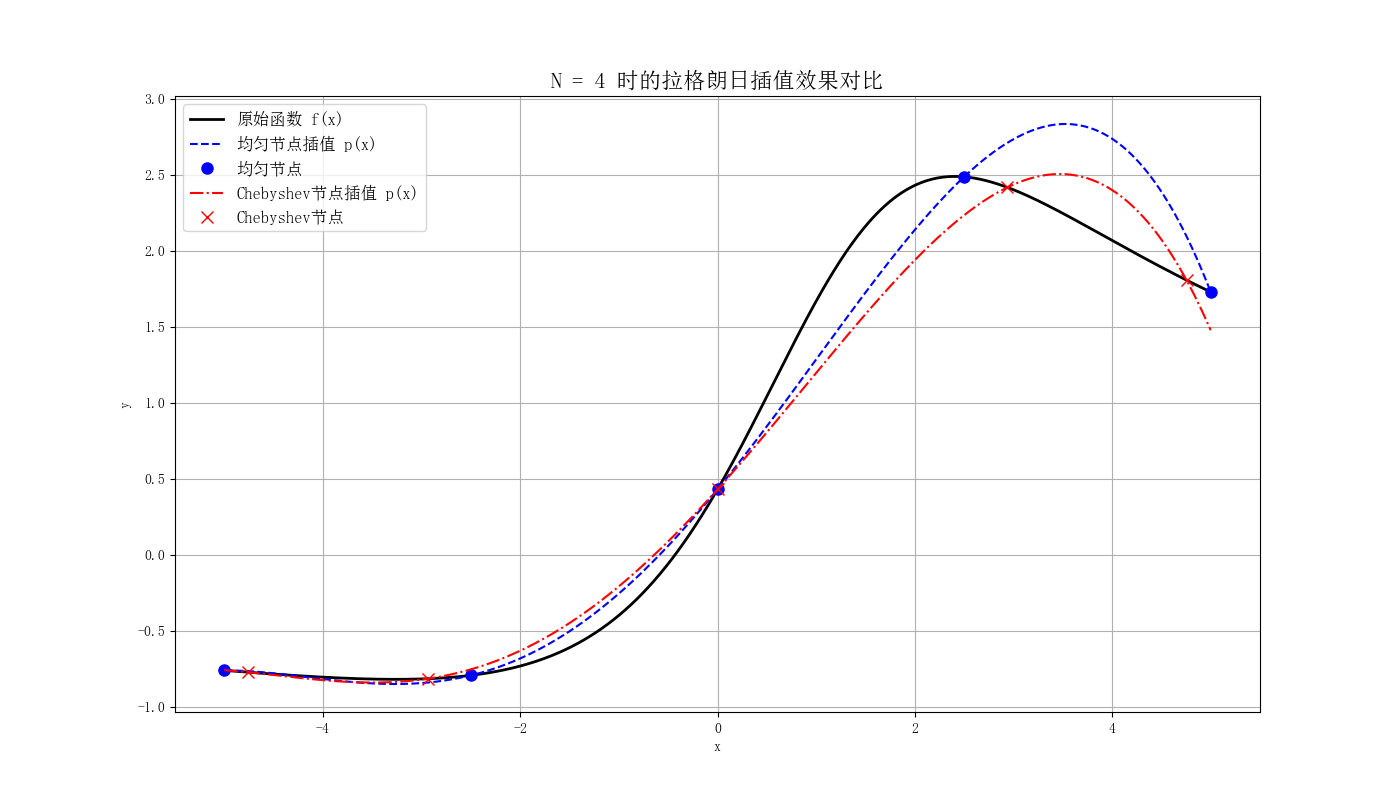
\includegraphics[width=0.9\textwidth]{n_4.png}
	\caption{N = 4 时的插值效果比较。}
	\label{fig:n4}
\end{figure}

\begin{figure}[H]
	\centering
	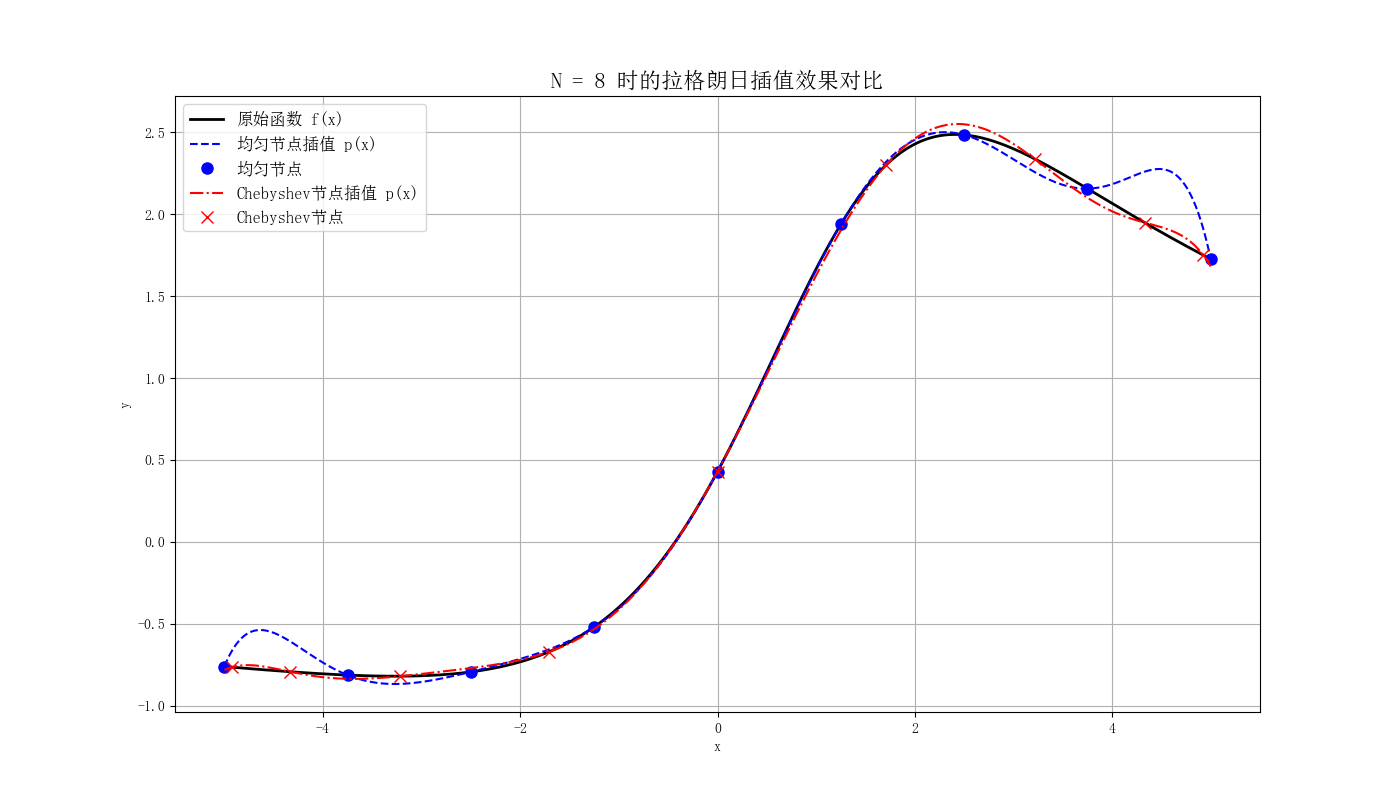
\includegraphics[width=0.9\textwidth]{n_8.png}
	\caption{N = 8 时的插值效果比较。}
	\label{fig:n8}
\end{figure}

\begin{figure}[H]
	\centering
	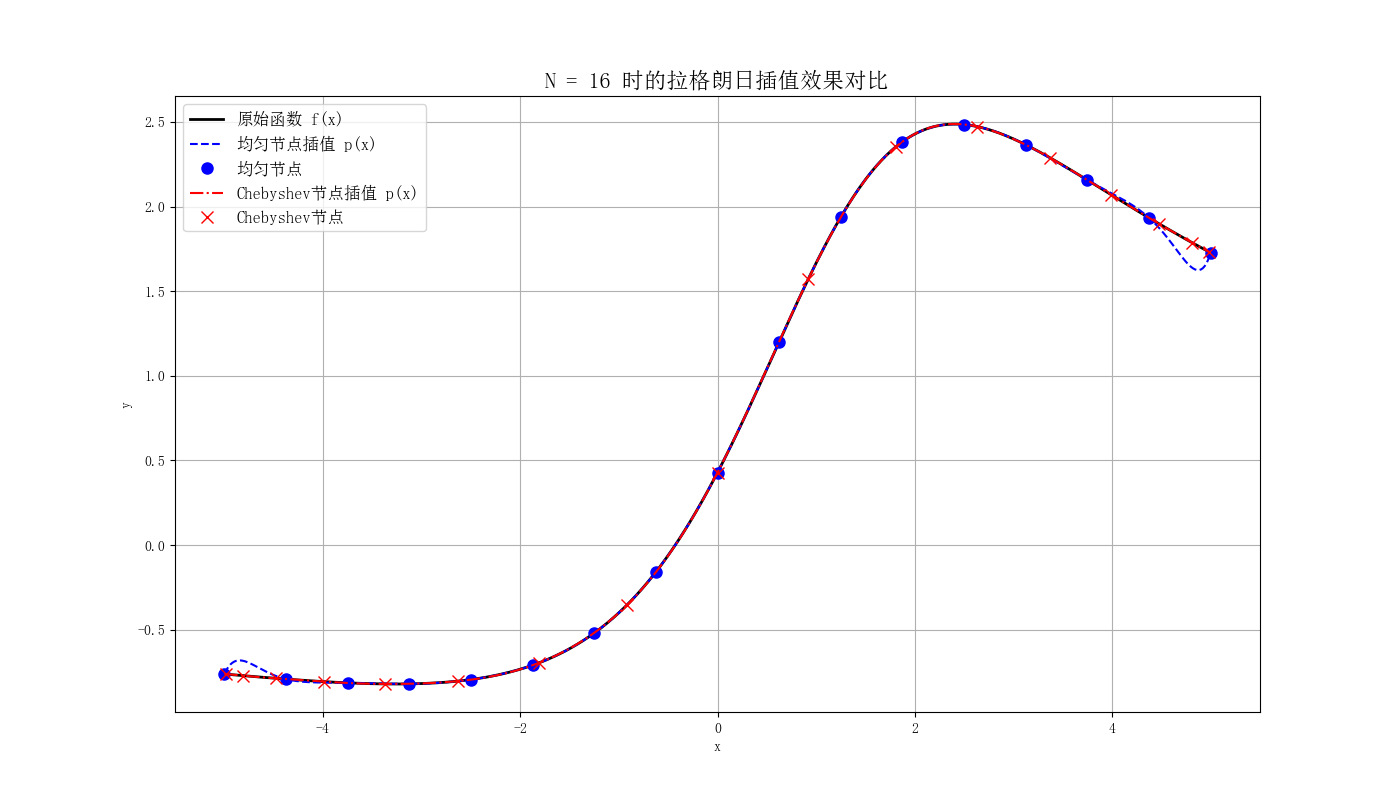
\includegraphics[width=0.9\textwidth]{n_16.png}
	\caption{N = 16 时的插值效果比较。}
	\label{fig:n16}
\end{figure}

\begin{figure}[H]
	\centering
	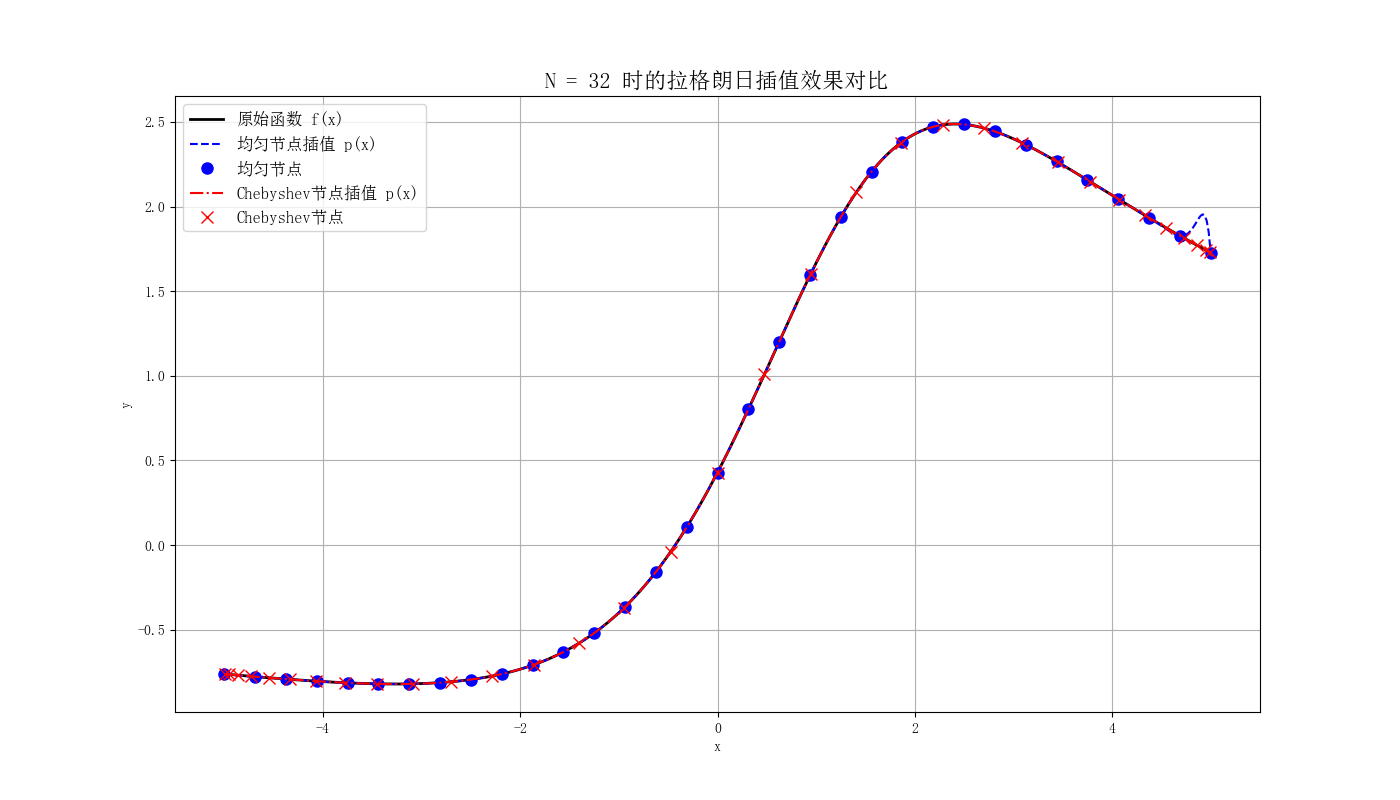
\includegraphics[width=0.9\textwidth]{n_32.png}
	\caption{N = 32 时的插值效果比较。}
	\label{fig:n32}
\end{figure}

	\begin{table}[H]
	\begin{center}
	\begin{tabular}{|c|c|c|}
	\hline
	$N$ & 均匀节点 & Chebyshev点 \\
	\hline
	$4$ & $6.709734906709E-01$ & $5.791068582057E-01$ \\
	\hline
	$8$ & $4.023793018811E-01$ & $6.462121535431E-02$ \\
	\hline
	$16$ & $1.486780140795E-01$ & $1.724881338690E-03$ \\
	\hline
	$32$ & $2.012959022700E-01$ & $7.322608591154E-07$ \\
	\hline
	\end{tabular}
	\end{center}
	\end{table}


\section{算法分析与结果分析}
本题要求实现拉格朗日多项式插值，并比较两种不同节点选取方式（均匀节点与切比雪夫节点）的插值效果。为此，程序首先定义目标函数 $f(x)$。根据题目中给定的公式，程序在主循环中针对 $N=4,8,16,32$ 分别生成了均匀分布和切比雪夫分布的 $N+1$ 个插值节点。

核心的插值计算部分，通过 \texttt{lagrange\_interpolation} 函数实现。该函数按照拉格朗日基函数的定义，对任意给定的 $x$ 值计算出对应的插值多项式 $p(x)$ 的值。最后，通过在 $[-5,5]$ 区间上进行密集采样，程序计算并记录了两种方法下插值多项式与原函数的最大误差，并绘制了对比图像。
实验结果表明，两种节点选取方式在插值效果上表现出巨大差异。对于均匀节点，随着插值次数 $N$ 的增加，插值误差并未单调减小。从数据表和图像 (图3, 图4) 可以清晰地看到，当 $N$ 较大时，插值多项式在区间两端与原函数产生巨大偏离，即Runge现象。相比之下，采用切比雪夫节点的插值误差则随着 $N$ 的增加而稳定、快速地减小，插值多项式在整个区间上都表现出良好的一致逼近效果，有效避免了Runge现象。

\section{实验小结}
本次数值实验通过对同一函数 $f(x)$ 施行拉格朗日插值，深刻揭示了插值节点的选取对高次多项式插值效果的决定性影响。实验结果清晰地表明，尽管均匀节点的选取方式直观简单，但在插值次数 $N$ 较高时，它会不可避免地导致剧烈的龙格现象，即插值多项式在区间两端产生剧烈振荡，致使误差不减反增，失去了近似的意义。与此形成鲜明对比的是，采用“两端密、中间疏”分布的切比雪夫节点，则能有效抑制这种振荡，使得插值多项式在整个区间上都能良好地逼近原函数。随着 $N$ 的增大，基于切比雪夫节点的插值误差能够稳定且快速地收敛，展现了其在数值计算中的优越性和可靠性。因此，本实验有力地证明了在进行高次多项式插值时，选择合适的非均匀节点（如切比雪夫节点）是保证算法收敛和获得高精度近似解的关键。

\end{document}